\documentclass[class=article,border=1pt]{standalone}
\usepackage[dvipsnames]{xcolor}
\usepackage{tikz}
\begin{document}
\pagestyle{empty}
\thispagestyle{empty}
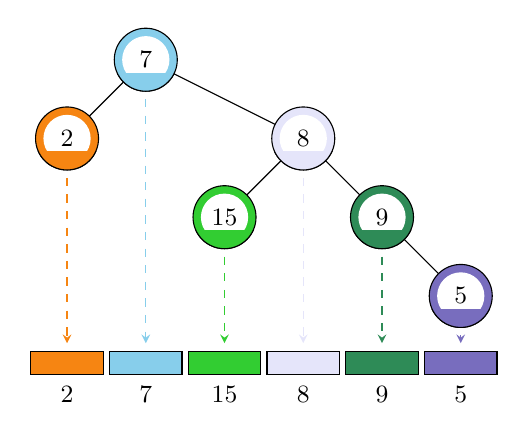
\begin{tikzpicture}
%   7
% 2      8
%     15   9
%            5
\draw ( 1, -0) -- ( 0, -1);
\draw ( 1, -0) -- ( 3, -1);
\draw ( 4, -2) -- ( 3, -1);
\draw ( 3, -1) -- ( 2, -2);
\draw ( 4, -2) -- ( 5, -3);
%
\newcommand{\vertex}[4]{
  \draw[->,>=stealth,dashed,draw=#3] (#1, #2 - 0.5) -- (#1, -3.6);

  \draw[fill=#3](#1, #2) ellipse (0.4 and 0.4);
  \draw[fill=white,draw=none] (#1, #2) ellipse (0.3 and 0.3);
  \begin{scope}
    \clip (#1-0.5,#2-0.5) rectangle (#1+0.5, #2-0.17);
    \draw[fill=#3] (#1, #2) ellipse (0.4 and 0.4);
  \end{scope}
  \node[anchor=center] at (#1, #2) {\small #4};

  \draw[fill=#3] (#1-0.46, -3.7) rectangle (#1+0.46, -4.0);
  \node[anchor=center] at (#1, -4.25) {\small #4};
}
%
\vertex{0}{-1}{BurntOrange}{2}
\vertex{1}{-0}{SkyBlue}{7}
\vertex{2}{-2}{LimeGreen}{15}
\vertex{3}{-1}{Lavender}{8}
\vertex{4}{-2}{SeaGreen}{9}
\vertex{5}{-3}{Periwinkle}{5}
%
\end{tikzpicture}
\end{document}
